\section{Getting started}
\label{sec:gstarted}

The necessary files are all in one directory.
The black box is in \texttt{blackbox.py} and can be run from the Python shell (Windows) or terminal (Linux). Using a terminal the following command runs the code,\\
\indent \texttt{python blackbox.py}

\noindent In order to run the GUI the \texttt{gui.py} file needs to in either the Python shell (Windows) or terminal (Linux). Using a termninal the following command runs the code,\\
\indent \texttt{python gui.py}\\
\begin{figure}[h]
%\centering
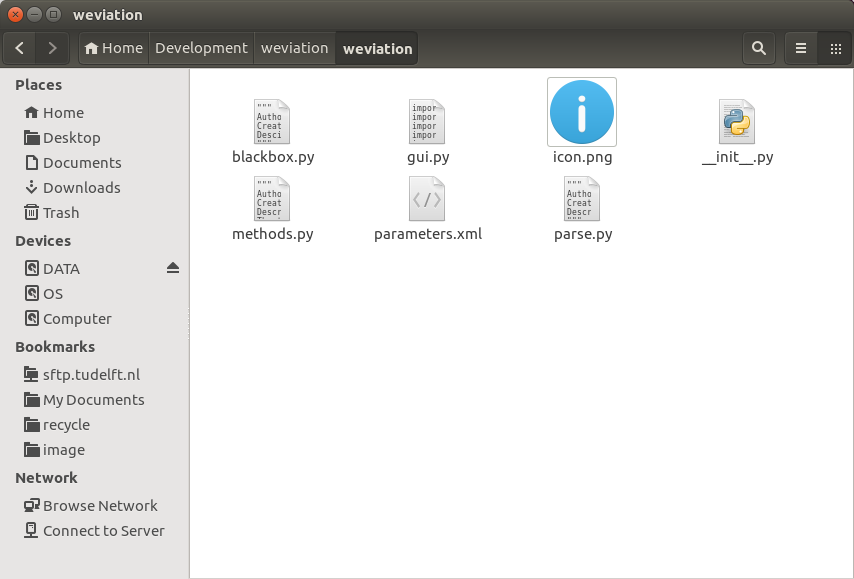
\includegraphics[width=0.5\textwidth]{image/directory.png}
\end{figure}

\subsection{Start up}
\noindent The figure below shows the GUI on start up and can be divided into three major sections: input data panel (red), the output panel (green) and visual output data (blue).

\begin{figure}[h]
%\centering
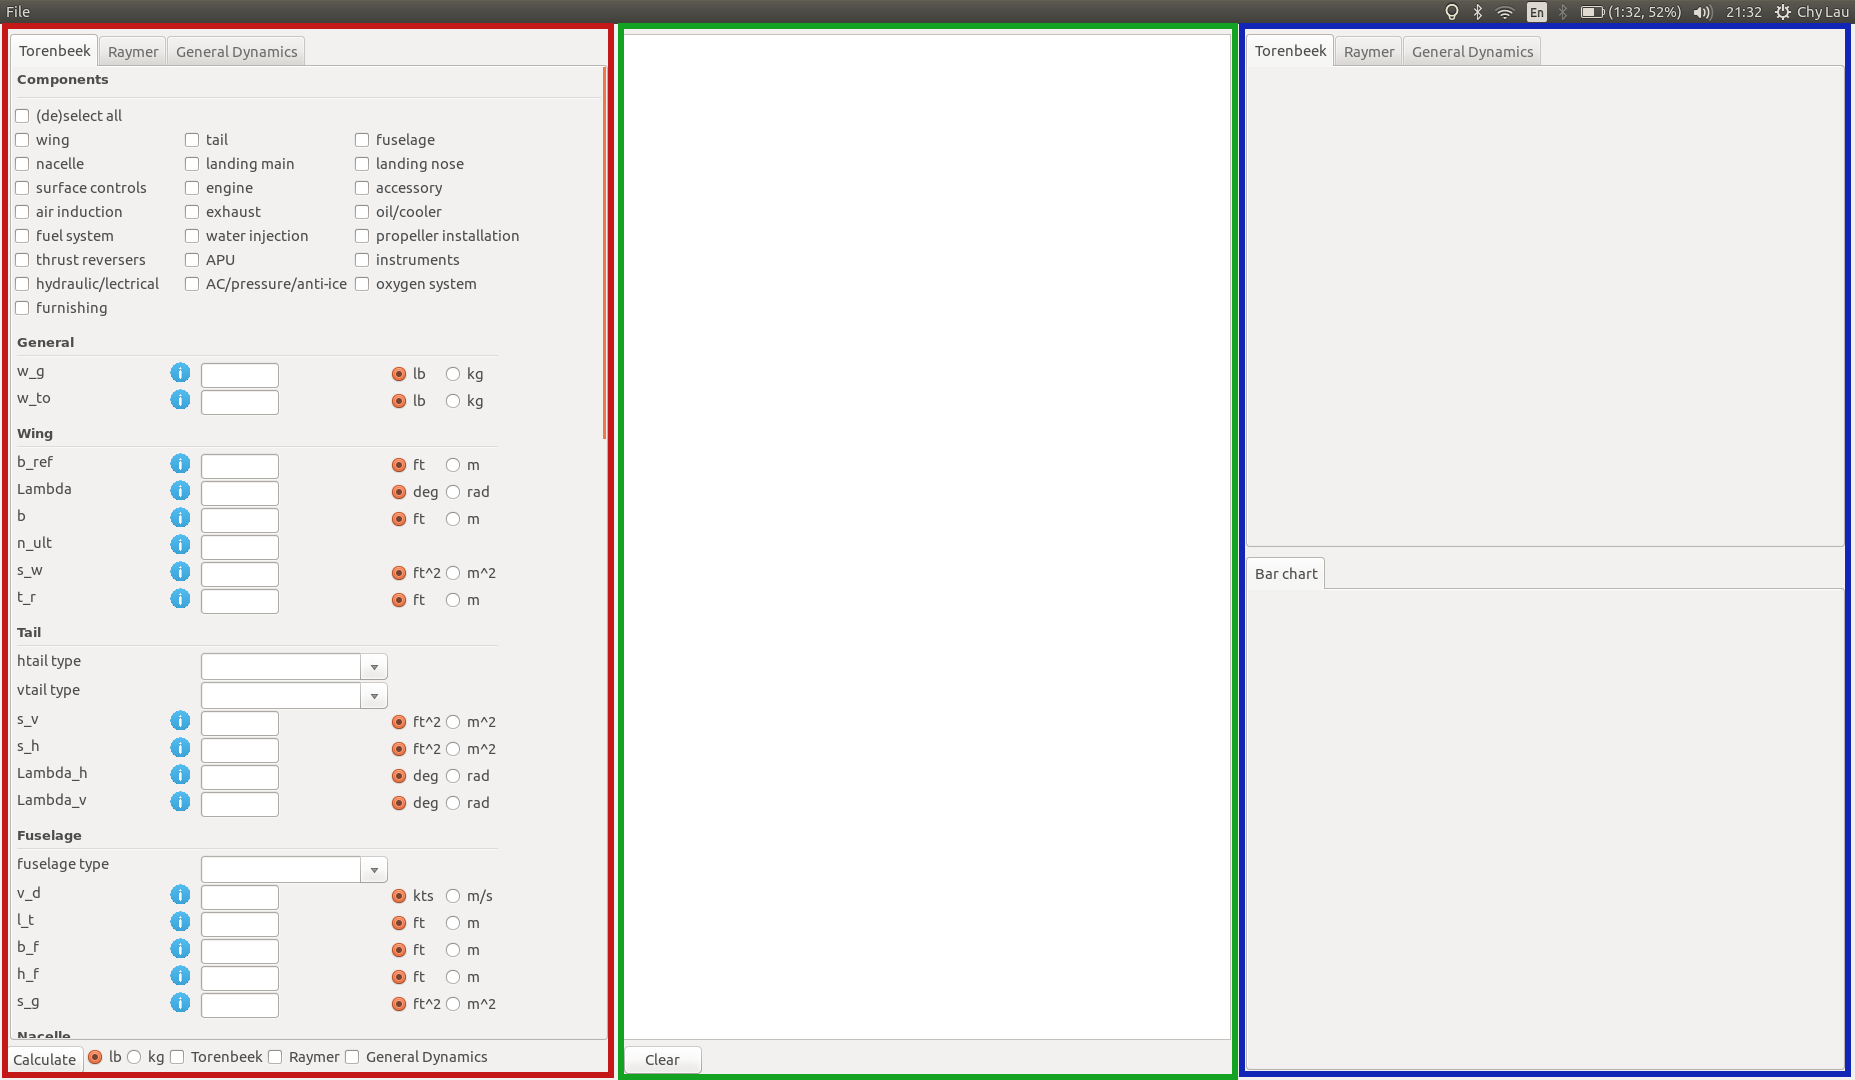
\includegraphics[width=0.9\textwidth]{image/gui_startup_colours.png}
\end{figure}

\clearpage
\subsection{Procedure}
\noindent In order to produce output data the following needs to be done:
\begin{enumerate}
    \item Selection of components (green): select which components you want to calculate of each method.
    \item Value input (purple): input the values of the parameters from the components that are selected.
    \item Unit system (orange): select in which unit system the input values are, either imperial or metric.
    \item Import XML file (yellow): under File in the menubar an XML file can be imported, which will automatically fill in the values.
    \item Calculate weights (red): select which methods you want to calculate and also the output data unit, again either imperial or metric; then click the calculate button.
    \item Export to XML/text (yellow): under File in the menubar the output data can be exported to XML or text file.
    \item Clear output data: to clear the output data panel, the clear button can be pressed. (\textbf{note:} when exporting the output data after clearing the panel, it will export the output data before clearing)
\end{enumerate}

\begin{figure}[ht]
%\centering
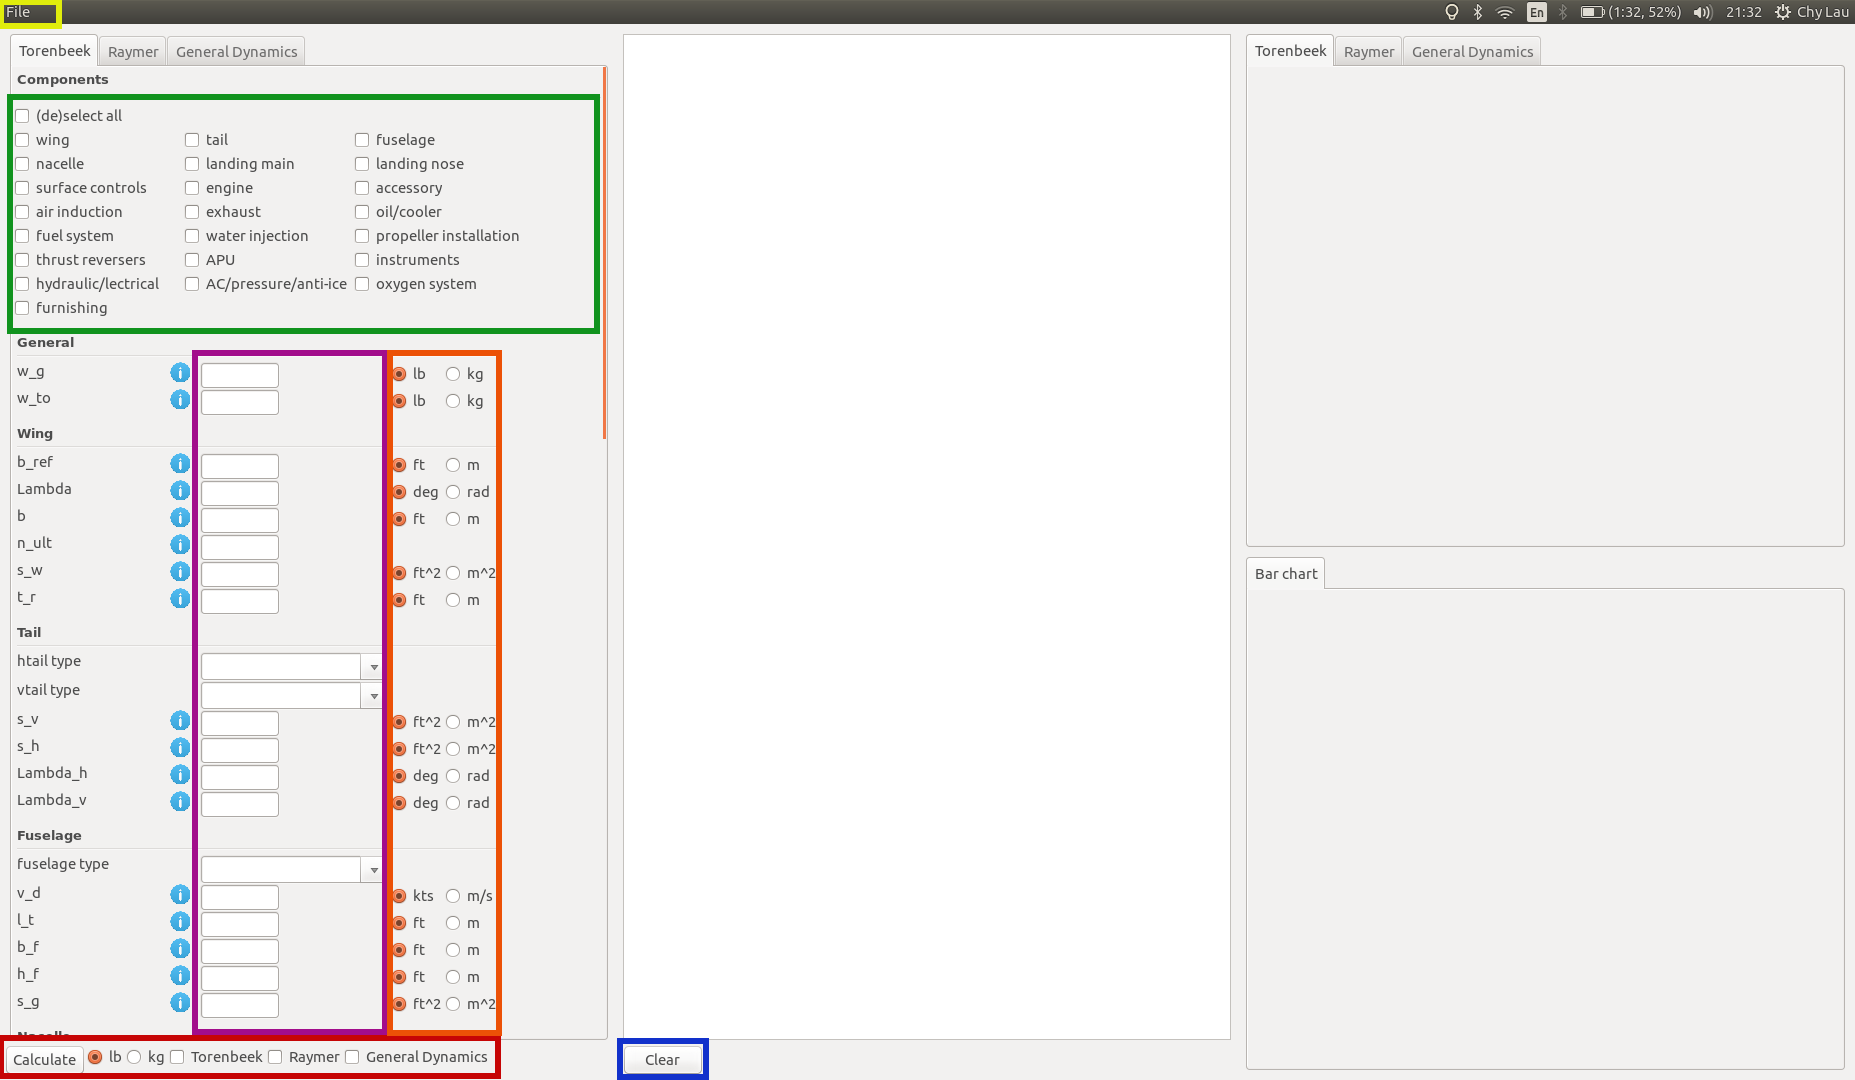
\includegraphics[width=1\textwidth]{image/gui_startup_boxes.png}
\end{figure}

\clearpage
\subsection{Tooltip}
\noindent Tooltips are added and are shown when the mouse hovers over the 
\includegraphics[scale=0.08]{image/icon.png} icon.
\begin{figure}[ht]
%\centering
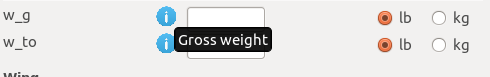
\includegraphics[width=0.5\textwidth]{image/gui_tooltip.png}
\end{figure}

\noindent For some parameters a value range is suggested.
\begin{figure}[h]
%\centering
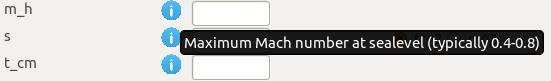
\includegraphics[width=0.5\textwidth]{image/gui_tooltip_typically.png}
\end{figure}

\subsection{Example output}
\noindent An example of a GUI with input and output parameters is shown below (\textbf{note:} these results showen below are not correct, and are purely for illustrative purposes).
The output data panel shows information of the aircraft and the results are structured into different groups.
When calculating multiple times, the results are appended, keeping the old results in the panel.

Next to each component name an abbreviation is given, which is used in the pie chart legend. In the pie chart the percentage of the total weight is shown for each component.

In the bar chart the total weight for each method is shown: Torenbeek (red bar), Raymer (green bar), General dynamics (blue bar).

\begin{figure}[ht]
%\centering
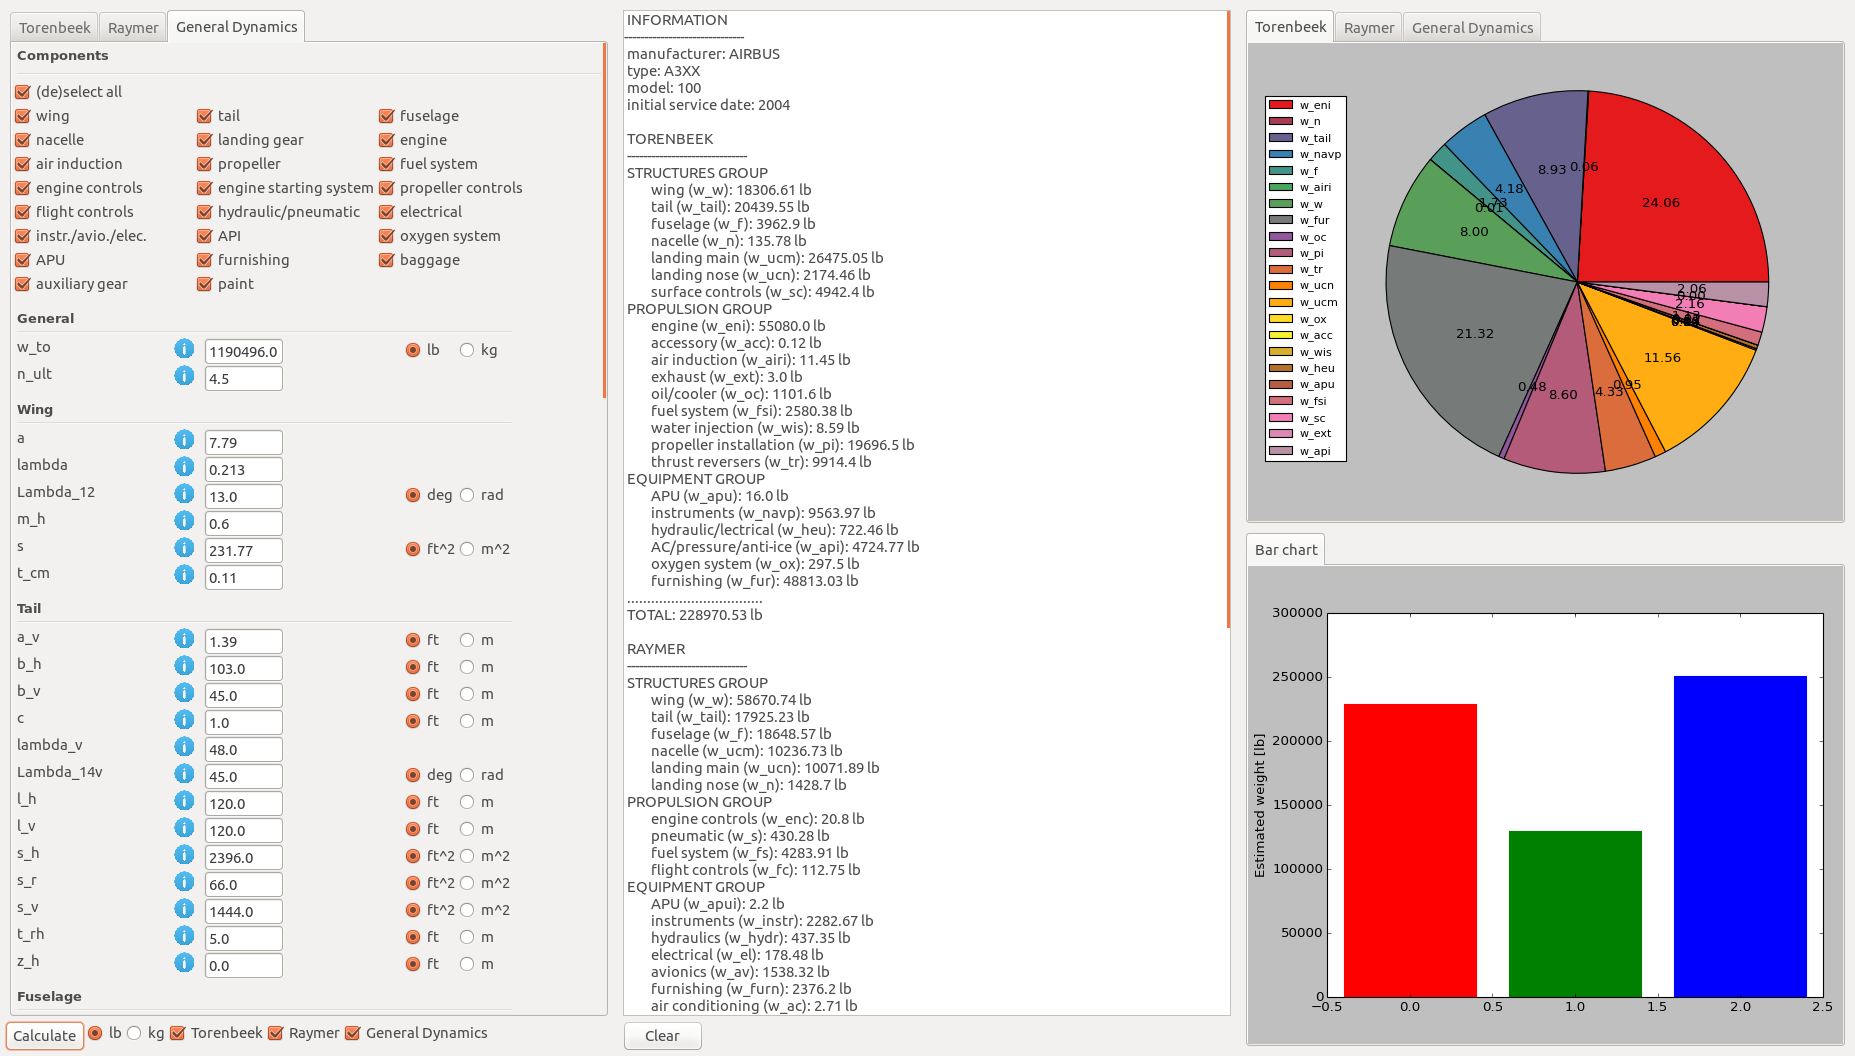
\includegraphics[width=1\textwidth]{image/gui_output.png}
\end{figure}
